\documentclass[10pt,pdf,hyperref={unicode}]{beamer}

% \documentclass[aspectratio=43]{beamer}
% \documentclass[aspectratio=1610]{beamer}
% \documentclass[aspectratio=169]{beamer}

\usepackage{lmodern}
\usepackage[T2A]{fontenc}
\usepackage[utf8]{inputenc}
\usepackage{tikz}
\usepackage[english,russian]{babel}
\addto{\captionsrussian}{
	\renewcommand{\figurename}{Рисунок}
}
\usepackage[labelsep=endash]{caption}


\graphicspath{{prez/}}

% отключить клавиши навигации
%\setbeamertemplate{navigation symbols}{}

\usetheme{Copenhagen}
\usecolortheme{default}

\title{Поиск вредоносной активности в DNS трафике}
 
\author{
	Студент: Меньших И.А.
	\and \\
	Руководитель: Солодушкин С.И.
}
\date{}

\begin{document}

% титульный слайд
\begin{frame}
\titlepage
\end{frame} 

\begin{frame}
\frametitle{Постановка задачи} 
Дано:
\begin{enumerate}
	\item DNS-логи
	\begin{enumerate}[-]
		\item source\_ip
		\item domain
		\item rcode
	
	\end{enumerate}
	\item Белый список (Alexa, Quancast)
	\item Черный список (SkyDNS)
\end{enumerate}

Необходимо:
\begin{enumerate}
	\item Найти вредоносные домены
	\item Выделить общие паттерны взаимодействия клиентов и вредоносных доменов
	\item Реализовать полученные подходы в виде программного кода и внедрить результат в производство
\end{enumerate}
\end{frame}

\begin{frame}
\frametitle{Обзор подходов} 
\begin{enumerate}
	\item Поэтапная фильтрация
	\item Анализ pDNS и WHOIS
	\item Sandbox + Reverse Engineering
	%\item <<Песочница>> и RE
\end{enumerate}
\end{frame}

\begin{frame}
\frametitle{Методы решения} 
\begin{enumerate}
	\item Групповая активность
	\item Ранжирование доменов
	\item Поиск и анализ паттернов взаимодействия
\end{enumerate}
\end{frame}

\begin{frame}
\frametitle{Групповая активность}
Предположения:
\begin{enumerate}
	\item Зараженных хостов в сети фиксированное количество.
	\item Взаимодействие зараженных хостов и C\&C сервера проявляется периодически.
	\item  Подозрительно, когда на один и тот же домен в разное время запрашивает узкий круг хостов.
\end{enumerate}
\end{frame}

\begin{frame}
\frametitle{Групповая активность}
Алгоритм поиска групповой активности
\begin{enumerate}
	\item Делим логи на <<окна>> фиксированного размера.
	\item Группируем хосты по домену.
	\item Фильтруем по черным/белым спискам и количеству уникальных пользователей.
	\item Сравниваем группы пользователей одного и того же домена в разных <<окнах>>, если группы сильно схожи - домен подозрительный.
\end{enumerate}
\end{frame}

\begin{frame}
\frametitle{Ранжирование доменов}
Идея - рассмотрим запросы пользователей за некоторый промежуток времени как граф.
\newline
\begin{definition}[Граф запросов]Двудольный неориентированный граф $(H\times D,  E)$, 
где $H$ - множество хостов, $D$ - множество доменных имён, ($h_i$, $d_j$)$\in$$E$, если пользователь $h_i$ запрашивал домен $d_j$. 
\end{definition}

\begin{figure}[H]
	\centering
	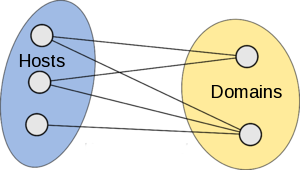
\includegraphics[scale=2.]{b_graph.png}
\end{figure}
\end{frame}


\begin{frame}
\frametitle{Ранжирование доменов}
Инициализируем начальные значения, опираясь на белый/черный список и итеративно будем вычислять оценки для доменов:
\begin{equation}
	\label{eq:dr1-black}
	black\_score(h_i) = \sum_{d_j: (h_i, d_j)\in E} \frac{black\_score(d_j)}{deg(d_j)}
\end{equation}
\begin{equation}
	\label{eq:dr1-white}
	white\_score(h_i) = \sum_{d_j: (h_i, d_j)\in E} \frac{white\_score(d_j)}{deg(d_j)}
\end{equation}
\begin{equation}
	\label{eq:dr1-union}
	union\_score(d_i) = \frac{black\_score(d_i)}{black\_score(d_i) + white\_score(d_i)}
\end{equation}
\begin{equation}
	\label{eq:dr2-rank}
	rank\_score(d_j) = \sum_{h_i: (h_i, d_j)\in E} \frac{rank\_score(h_i)}{deg'(h_i)}
\end{equation}
\end{frame}


\begin{frame}
\frametitle{Ранжирование доменов}
@@ВОТ ТУТ НУЖЕН ПРИМЕР, АНИМАЦИЯ
\end{frame}

\begin{frame}
\frametitle{Анализ паттернов взаимодействия}
Идея - рассматривать в графе только ребра, соответствующие неудачным запросам и искать <<плотные>> подграфы
\begin{figure}[H]
	\centering
	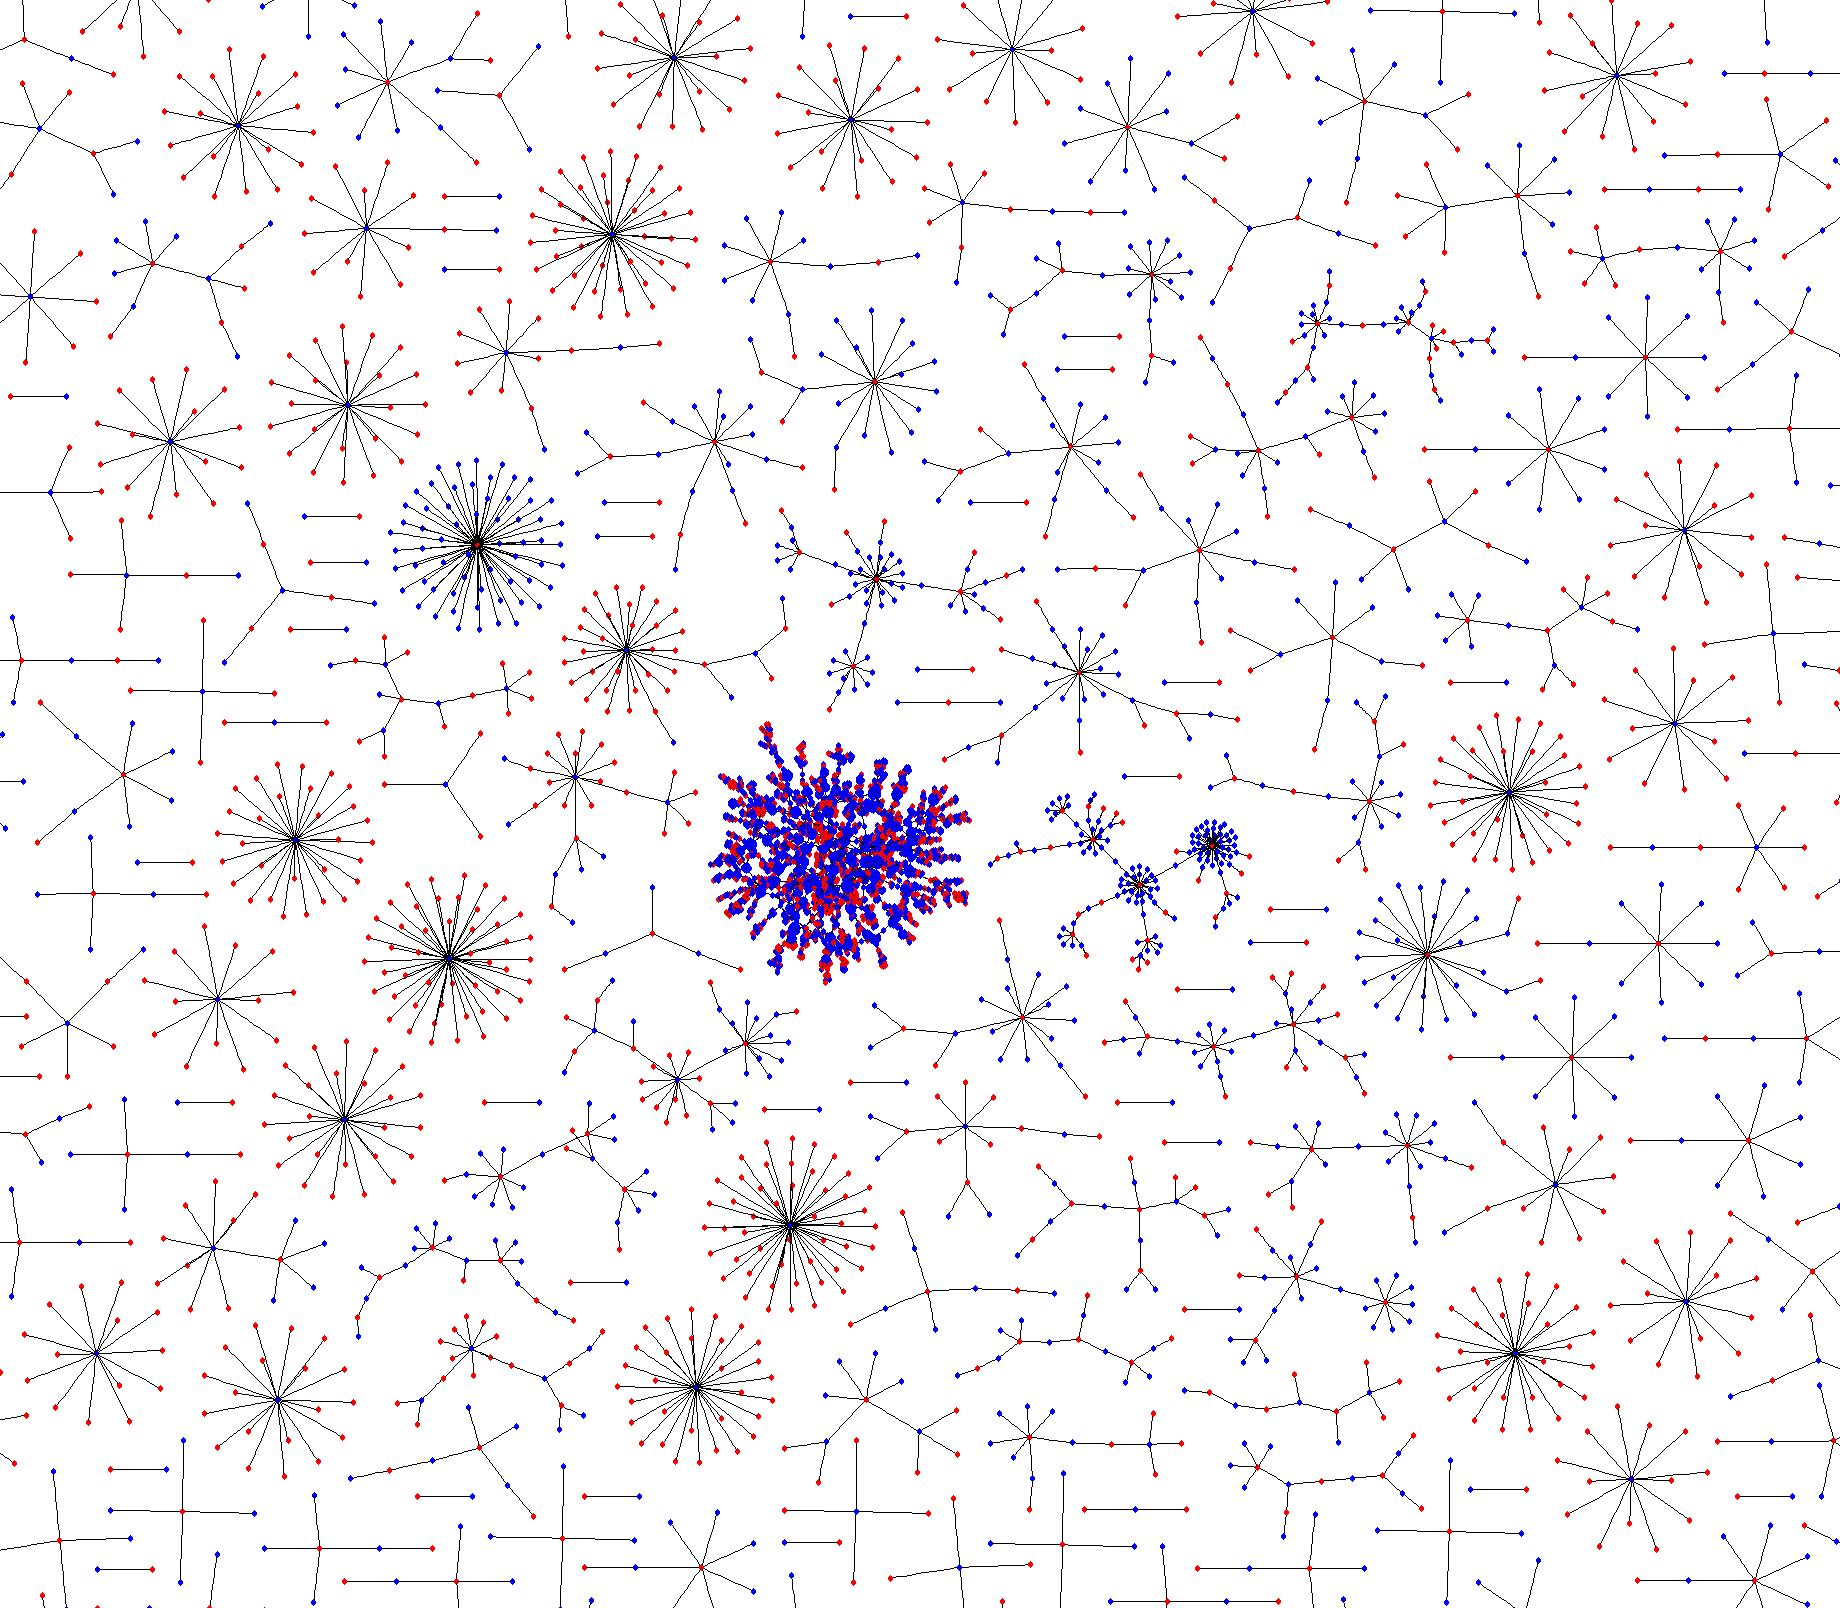
\includegraphics[scale=0.14]{img/fail-graph.png}
	\caption{Граф неудачных DNS-запросов (\tikz{\draw[fill=blue] (0,0) circle (0.1cm);} - хосты, \tikz{\draw[fill=red] (0,0) circle (0.1cm);} - домены)}
\end{figure}
\end{frame}

\begin{frame}
\frametitle{Анализ паттернов взаимодействия}
Алгоритм декомпозиции графа
\begin{enumerate}
	\item Удаляем ребра (DNS-Overload, SERVFAIL, etc)
	\item Находим все компоненты связности (BFS)
	\item Для каждой компоненты связности
	\begin{enumerate}
		\item Ищем плотные подграфы (3-NMF)
		\item Вычисляем $$density = \frac{|E|}{|H|*|D|}$$
		\item Удаляем те подграфы, которые либо маленькие, либо недостаточно <<плотные>>
	\end{enumerate}
\end{enumerate}
\end{frame}

\begin{frame}
\frametitle{Анализ паттернов взаимодействия}
@@ И тут нужен пример
\end{frame}

\begin{frame}
\frametitle{Объединение подходов и автоматизация анализа}
\begin{figure}[H]
	\centering
	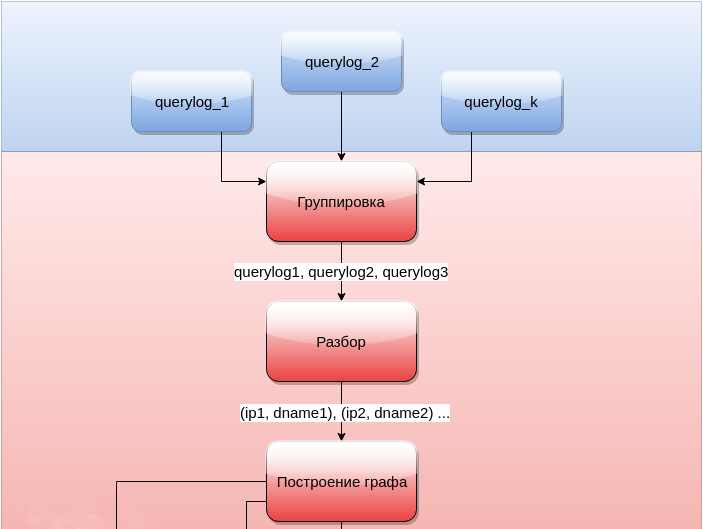
\includegraphics[scale=0.4]{schema-head.png}
\end{figure}
\end{frame}

\begin{frame}
\frametitle{Объединение подходов и автоматизация анализа}
\begin{figure}[H]
	\centering
	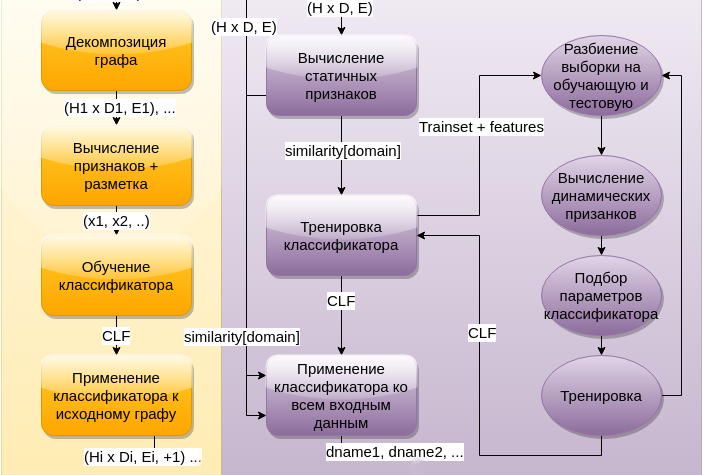
\includegraphics[scale=0.4]{schema-tail.png}
\end{figure}
\end{frame}

\begin{frame}
\frametitle{Итоги}
Результаты:
\begin{enumerate}
	\item Разработан программный продукт, который занимается поиском вредоносных доменов.
	\item Продукт внедрен в эксплуатацию в компании SkyDNS и показывает хорошие результаты в <<реальных>> условиях.
	\item Разработана основная часть системы для ручного анализа вредоносных подграфов.
\end{enumerate}

Что дальше:
\begin{enumerate}
	\item Продолжать работу над анализом <<плотных>> подграфов, автоматизировать этот процесс за счет дополнительной информации о доменах.
	\item Улучшать текущий анализатор за счет более тонкой настройки на этапе подбора параметров.
	
\end{enumerate}
\end{frame}

\begin{frame}
\frametitle{Благодарность}
\Large\centeringСпасибо за внимание!
\end{frame}





\end{document}